%
% Copyright (c) 2017  Zubax Robotics OU  <info@zubax.com>
%
% Distributed under BY-NC-ND (attribution required, non-commercial use only, no derivatives).
%

\documentclass{zubaxdoc}
\graphicspath{{document_templates/documentation_template_latex/}}

\usepackage{ConfigParamIndex}
\usepackage{makecell}
\usepackage{amsmath}

\title{Zubax GNSS 2 Datasheet}

\begin{document}
\frontmatter

\begin{titlepage}

\section*{Overview}

Zubax~GNSS~2 is a multipurpose high-performance positioning module interfaced via CAN bus, USB, and UART.
It includes a state-of-the-art multi-system GPS/\allowbreak{}GLONASS receiver,
a high-precision barometric altimeter, and a 3-axis compass with thermal compensation.

\section*{Features}

\begin{itemize}
    \item State-of-the-art concurrent GPS/GLONASS receiver u-blox MAX-M8Q.
    \begin{itemize}
    	\item Full RF shielding of the GNSS circuits ensures reliable operation in high-EMI environments.
    	\item 35 mm high-gain patch antenna with large ground plane for reliable reception even in deep urban canyons.
    	\item Analog front-end with LNA and SAW ensures high noise resilience.
    	\item Supercapacitor-based backup power source enables low time-to-first-fix (a few seconds).
    	\item Up to 15 Hz update rate.
    \end{itemize}
	\item High precision digital barometer TE Connectivity MS5611.
    \item High precision 3-axis digital compass STMicroelectronics LIS3MDL with thermal compensation.
	\item Supported interfaces:
    \begin{itemize}
        \item CAN, with optional double redundancy.
        \item UART.
        \item USB port, no drivers needed.
    \end{itemize}
    \item High quality assurance:
    \begin{itemize}
        \item Every manufactured unit undergoes a strict testing procedure.
        The testing log for each produced unit is available to the user via the website at\\
        \url{https://device.zubax.com/device_info}.
        \item Protection against unlicensed (counterfeit) production by means of a digital signature
        installed on every manufactured unit.
    \end{itemize}
\end{itemize}

\BeginRightColumn

\section*{Applications}

\begin{itemize}
	\item Positioning module for unmanned vehicles (aerial, ground, underwater, etc) and robots.
    \item General-purpose embedded positioning module.
\end{itemize}

\centering
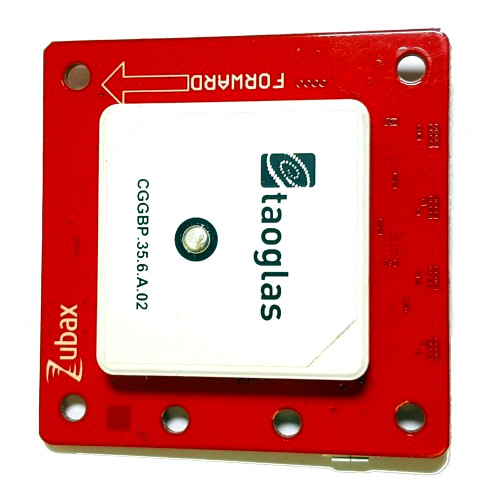
\includegraphics[width=0.45\textwidth]{GNSS_top}
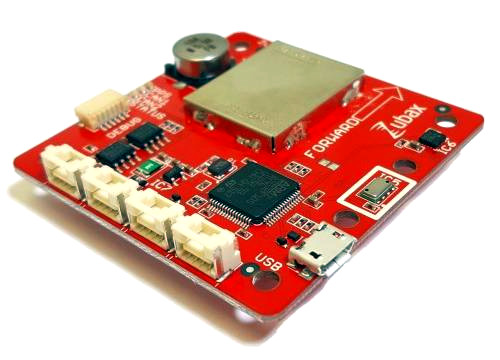
\includegraphics[width=0.45\textwidth]{GNSS_bottom}
\end{titlepage}

\tableofcontents
\clearpage
\listoftables
\listoffigures

\mainmatter

\chapter{Overview}

Zubax~GNSS~2 is a multipurpose high-performance positioning module interfaced via CAN bus, USB, and UART.
It includes a state-of-the-art multi-system GPS/GLONASS receiver, a high-precision barometric altimeter, and a 3-axis compass with thermal compensation.
Zubax~GNSS~2 supports a variety of standard protocols, which ensures compatibility with third party software and hardware: UAVCAN (over CAN bus), NMEA 0183 (over USB and UART), and the u-Blox M8 binary protocol.

\section{Accessories}

Zubax~GNSS~2 can be used with the following accessories:

\begin{itemize}
    \item Plastic enclosure described in the section \ref{sec:enclosure}.
    \item UAVCAN cabling and related items. Refer to \url{https://kb.zubax.com/x/EoAh} for more information.
    \item Zubax Dronecode probe. Refer to \url{https://kb.zubax.com/x/iIAh} for more information.
\end{itemize}

Please contact your supplier for ordering information.

\subsection{Enclosure}\label{sec:enclosure}

Zubax~GNSS~2 is intended for integration into the end system in the form of the bare PCB,
as this facilitates lower weight and tighter arrangement of components
in the end device, all of which are desirable properties in the target application domains.

Shall it be desired to provide additional mechanical protection for the device or to install it away from possible sources of electromagnetic interference, the plastic components pictured on the figure \ref{enclosure} can be used.
Please contact your supplier for the ordering information;
alternatively, visit \url{https://github.com/Zubax/zubax_gnss} to download
the 3D printable models suitable for in-house manufacturing.

\begin{figure}[hbt]
	\centering
	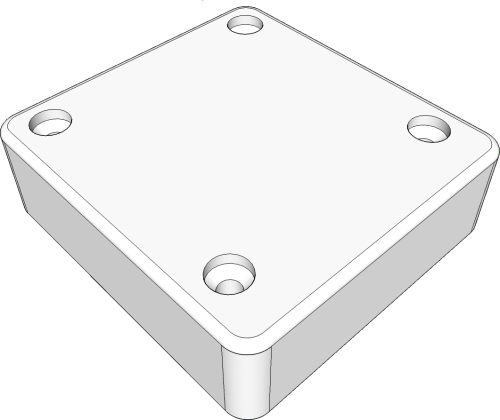
\includegraphics[width=0.45\textwidth]{enclosure_assembled_top}
	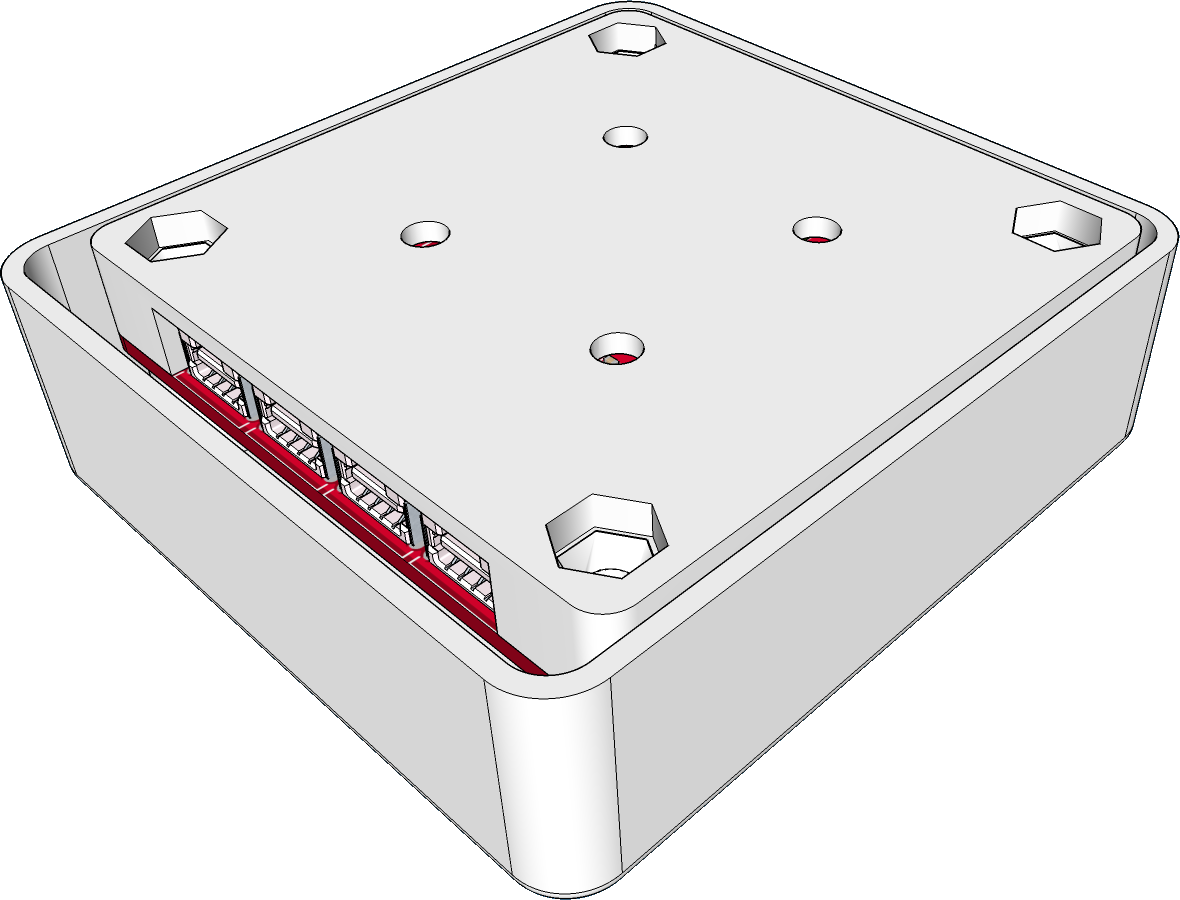
\includegraphics[width=0.45\textwidth]{enclosure_assembled_bottom}
	\caption{Plastic enclosure suitable for 3D-printing, top and bottom, assembled.\label{enclosure}}
\end{figure}

\begin{figure}[hbt]
	\centering
	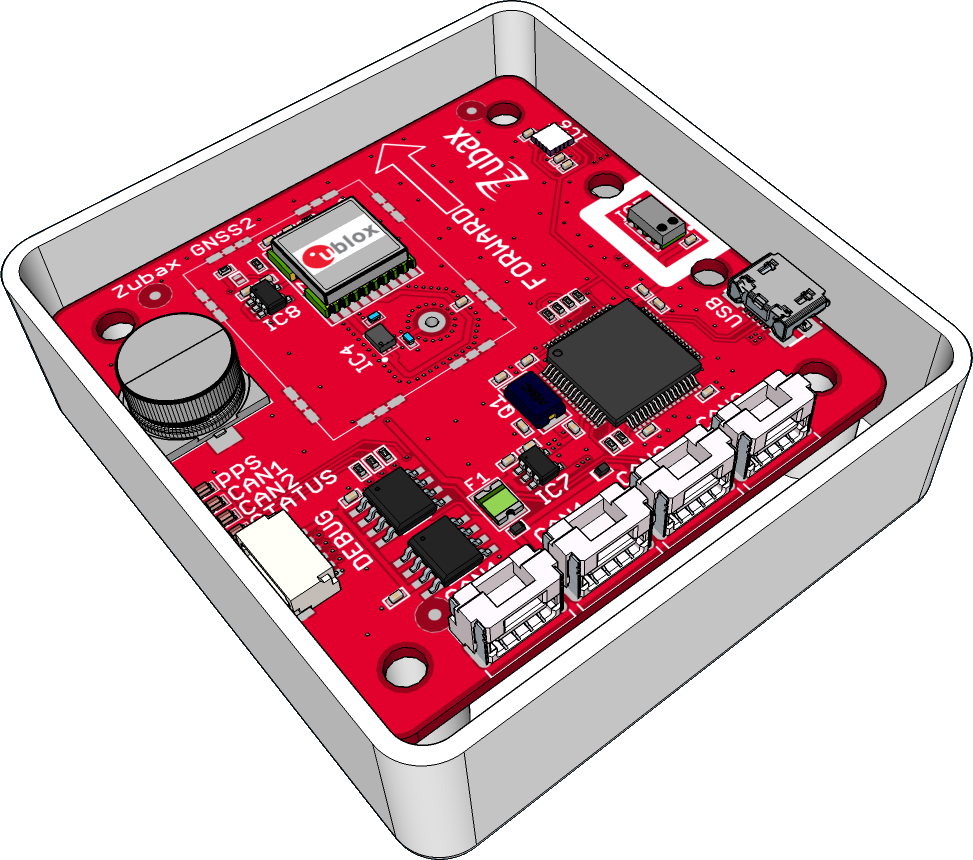
\includegraphics[width=0.45\textwidth]{enclosure_pcb_top}
	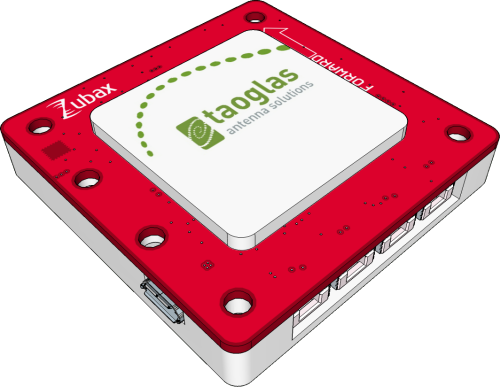
\includegraphics[width=0.45\textwidth]{enclosure_pcb_bottom}
	\caption{Top and bottom parts of the enclosure with the device inside.}
\end{figure}

\section{Quality assurance}

Every manufactured Zubax~GNSS~2 undergoes an automated testing procedure that validates that
the device is functioning as designed.
The test log for every manufactured device is available on the web at
\url{https://device.zubax.com/device_info}.
This feature can be used to facilitate traceability of purchased devices and
provide additional safety assurances.

Besides testing, every manufactured device has a digital signature installed,
that can be used as a strong protection against unlicensed or counterfeit manufacturing.
Please contact Zubax Robotics
to find out the specifics about digital signature verification.

\chapter{Characteristics}

\section{Absolute maximum ratings}

Subjecting the device to stresses beyond those specified in this section may cause
permanent damage to the device.
Proper operation of the device within the ranges specified in this section is not implied.

\begin{ZubaxSimpleTable}{Absolute maximum ratings}{|c X|c c|c|}
    Symbol            & Parameter                & Min  & Max & Unit \\
	$V_\text{supply}$ & Supply voltage           & -0.3 & 6   & V \\
	$T_\text{oper}$   & Operating temperature    & -40  & 105 & \degree{}C \\
	                  & UART input voltage 		 & -0.3 & 6   & V\\
	                  & CAN H/L input voltage    & -4   & 16  & V\\
\end{ZubaxSimpleTable}

\section{Environmental conditions}\label{environmental_conditions}

The GNSS hot start feature is not expected to work reliably below -20\degree{}C
due to poor performance of the supercapacitor-based backup power source at low temperatures.
However, this should not have any adverse side effects on the general performance of
the unit except that the time-to-first-fix (TTFF) may be higher than normal.

Magnetic fields whose magnitude exceeds the limit may render the compass temporarily dysfunctional.
Other components are unlikely to be affected.

\begin{ZubaxTableWrapper}{Environmental conditions}
    \begin{ZubaxWrappedTable}{|c X|l c|c|c|}
        Symbol            & Parameter                     &  Min & Max & Unit \\
        $T_\text{oper}$   & Operating temperature         & -40  & 100 & \degree{}C \\
        $B$               & Magnetic field strength       &      & 9   & Gauss \\
        $\phi_\text{oper}$& Operating humidity\tnote{1}   & 0    & 100 & \%RH\\
        $h_\text{oper}$   & Operating altitude above mean sea level (MSL) &     & 10  & km\\
    \end{ZubaxWrappedTable}
    \begin{tablenotes}
        \item[1] Condensation not permitted.
    \end{tablenotes}
\end{ZubaxTableWrapper}

\section{Reliability}

Please contact Zubax Robotics for additional reliability and safety information.

\begin{ZubaxSimpleTable}{Reliability}{|c X|c|c|}
    Symbol & Parameter & Typ & Unit \\
	MTTF   & Mean time to failure & 500000 & hours \\
\end{ZubaxSimpleTable}

\section{Sensor suite}

\subsection{GNSS receiver}

The device employs the \textbf{u-Blox MAX-M8Q} GNSS receiver module.
Please refer to the specifications provided by u-Blox to gain additional information about the module.

The internal delay (lag) of the GNSS receiver is approximately 200 milliseconds.

The period of GNSS solution reporting is defined by the configuration parameters
\CfgRef{uavcan.pubp-fix} and \CfgRef{uavcan.pubp-aux}, in microseconds.

The parameters \CfgRef{gnss.warn+dimens} and \CfgRef{gnss.warn+sats} can be used to reflect the quality of
the GNSS solution in the device health code.

\subsection{Digital barometric altimeter}

The device employs the \textbf{TE Connectivity MS5611} digital barometric altimeter.
Please refer to the specifications provided by TE Connectivity to gain additional information about the sensor.

The measurement period (which equals the reporting period) is defined by the configuration parameter 
\CfgRef{uavcan.pubp-pres}, in microseconds.
The reported error variances for pressure and temperature estimates are defined by the parameters
\CfgRef{pres.variance}, in $\text{pascal}^2$, and \CfgRef{temp.variance}, in $\text{kelvin}^2$,
respectively.

\subsection{Three-axis digital compass with thermal compensation}

The device employs the \textbf{STMicroelectronics LIS3MDL} digital three-axis compass with thermal compensation.
Please refer to the specifications provided by STMicroelectronics to gain additional information about the sensor.

Zubax GNSS v2.1 and older (manufacturing years 2015--2016) used to employ \textbf{Honeywell HMC5983} instead.
These modifications of the hardware are no longer manufactured.

The measurement period (which equals the reporting period) is defined by the configuration parameter 
\CfgRef{uavcan.pubp-mag}, in microseconds.
The reported error variance for magnetic field strength measurements is defined by the parameter
\CfgRef{mag.variance}, in $\text{gauss}^2$.

The measured magnetic field vector can be rescaled with the help of the parameter \CfgRef{mag.scaling+coef}.
This feature can be used to work-around magnetic field scaling issues in some commercial UAV autopilots.

The parameter \CfgRef{mag.pwron+slftst} can be used to control whether the magnetic field sensor should be
subjected to a self-test when the device is powered on.\footnote{Available for hardware v2.2 and newer.}
This feature must be disabled if the device is expected to be powered on while non-stationary,
otherwise false failures may be detected.

\section{Communication interfaces}

Zubax~GNSS~2 features three communication interfaces. Each is described in detail in the subsequent parts of this document.
\begin {itemize}
\item Doubly redundant UAVCAN interface with two connectors for each interface.
\item USB port.
\item Dronecode port.
\end{itemize}

\subsection{CAN bus interface}

This interface provides full access to all features of Zubax~GNSS~2, including the output of measurements,
reconfiguration, time synchronization, firmware update, etc.

Zubax~GNSS~2 is equipped with a doubly-redundant CAN bus interface, which can be used in the non-redundant mode
as well.
Each of the interfaces is equipped with two standard
UAVCAN Micro connectors (JST GH)\footnote{\url{https://kb.zubax.com/x/EoAh}}
electrically parallel to each other,
which facilitates easy integration of the device into the end application without the need to use T-connectors.

\subsubsection{Device interconnection}

Zubax~GNSS~2 can be used with doubly-redundant and non-redundant CAN buses.
In the latter case, only CAN1 can be used, and CAN2 must be left unconnected.
The figure \ref{can_daisy_chain} shows the possible device interconnection schemes.

\begin{figure}[hbt]
    \center
	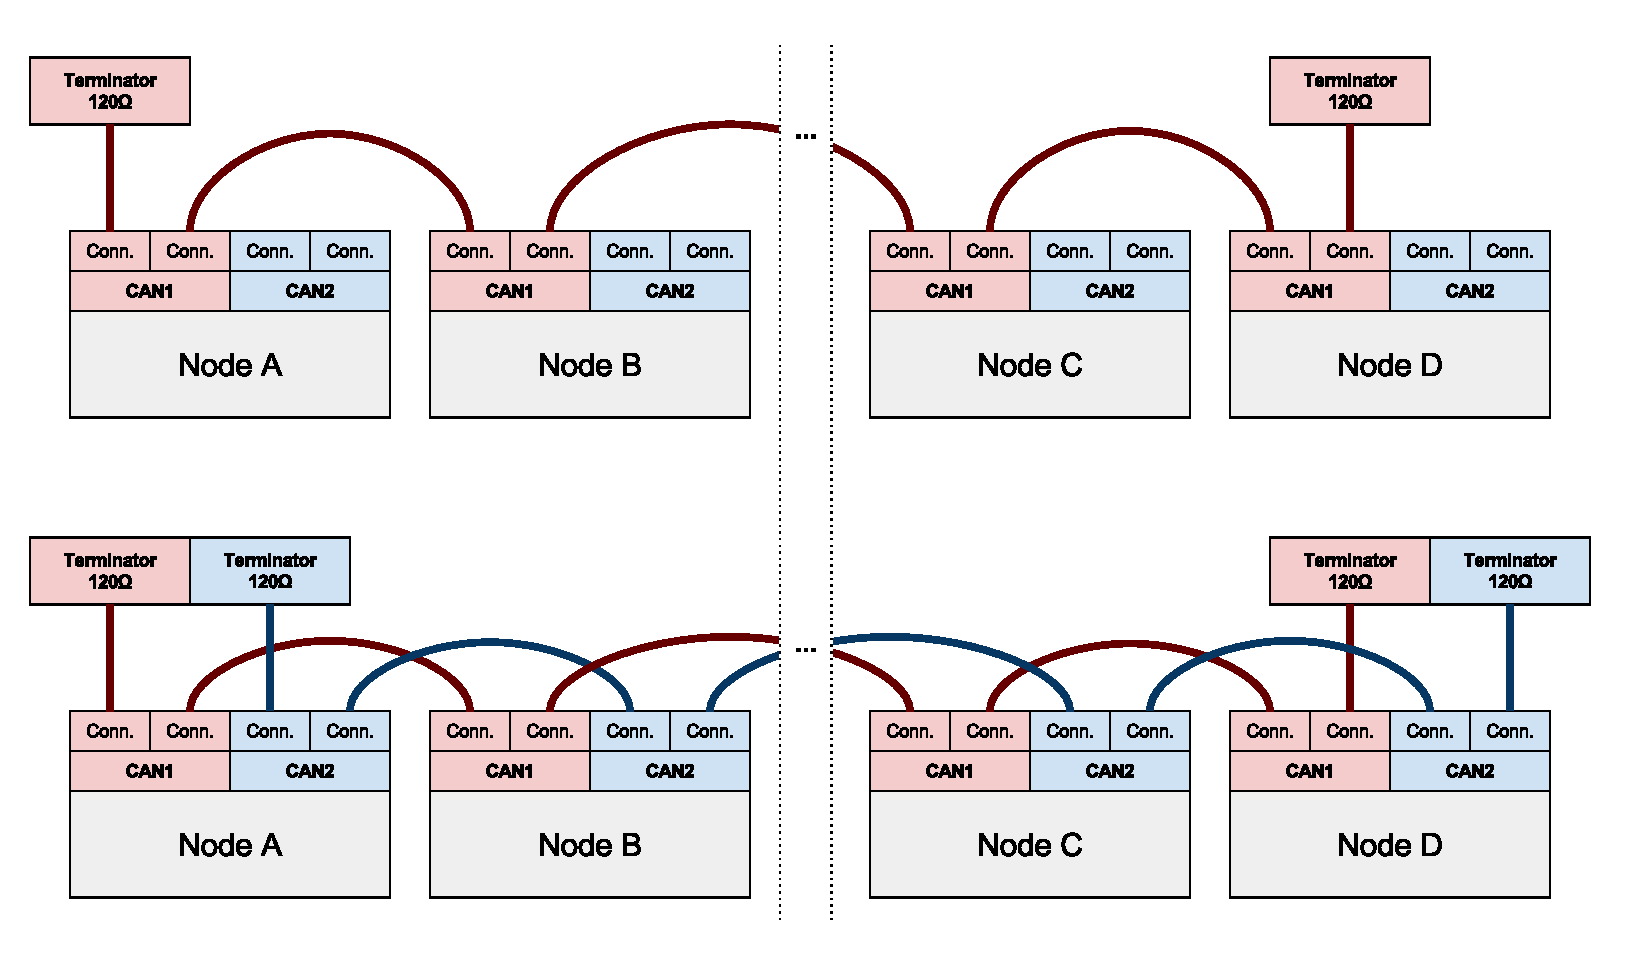
\includegraphics[width=1\textwidth]{can_daisy_chain}
	\caption{CAN bus interconnection diagram for non-redundant and a doubly-redundant interfaces.
	\label{can_daisy_chain}}
\end{figure}

\subsubsection{Connector pinout}

\begin{ZubaxTableWrapper}{UAVCAN Micro (JST GH) standard connector pinout}
    \begin{ZubaxWrappedTable}{|l X X[2]|}
        Pin no. & Type            & Function\\
        1       & Power           & +5 V power supply input and pass-trough\\
        2       & Input/output    & CAN High\\
        3       & Input/output    & CAN Low\\
        4       & Ground          & Power \& signal ground\\
    \end{ZubaxWrappedTable}
\end{ZubaxTableWrapper}

\subsubsection{Physical characteristics}

\begin{ZubaxTableWrapper}{Characteristics of CAN bus interfaces}
	\begin{ZubaxWrappedTable}{|c X|c c c|c|}
		Symbol  & Parameter                                 & Min  & Typ  & Max  & Unit \\
		        & Bit rate                                  & 20   &      & 1000 & Kbps \\
		        & Positive-going input threshold voltage    &      & 750  & 900  & mV \\
		        & Negative-going input threshold voltage    & 500  & 600  &      & mV \\
		        & Differential output voltage, dominant     & 1.5  & 2.0  & 3.0  & V \\
		        & Differential output voltage, recessive    & -120 & 0    & 12   & mV \\
		        & Inter-connector current pass-through\tnote{1}& -1&      & 1    & A \\
		        & Connector resistance during device lifetime &    & 30   & 50   & $\text{m}\Omega$ \\
	\end{ZubaxWrappedTable}
	\begin{tablenotes}
	    \item [1] The limit is imposed by the PCB.
	\end{tablenotes}
\end{ZubaxTableWrapper}

\subsection{USB interface}

The device implements a full-speed USB 2.0 port with the standard CDC ACM interface
(also known as ``virtual serial port'').
The device features driverless compatibility with all major operating systems
(Windows, GNU/Linux, Mac OS).\footnote{Get more knowledge and helpful tips at \url{https://kb.zubax.com}.}

The physical connector type is USB micro B (which is the most common device-side USB connector type).

\subsubsection{Protocol selection}

The following protocols are exposed via the USB interface:
\begin{description}

    \item[NMEA 0183] Used to output measurements in the industry-standard NMEA 0183 protocol.
    This protocol is enabled only if the virtual serial port is opened with a baud rate value in the
    range from 4800 to 57600 baud/second, inclusive.
    More information about the NMEA protocol is provided in the section \ref{nmea_output}.

    \item[CLI] The command-line interface provides access to the device's management and diagnostic
    features. This protocol is always enabled; however, it is not expected to be practically useful
    while used in parallel with other protocols, such as NMEA.
    More information about the CLI is provided in the section \ref{command-line_interface}.

\end{description}

Observe that unlike many other implementations of virtual serial ports,
this implementation is sensitive to the baud rate setting,
because it is used by the device to detect whether the NMEA output should be enabled.
The rationale behind this logic is to facilitate compatibility with third party software products.

Many legacy GNSS receivers equipped with physical UART interfaces emit NMEA data at very low
baud rates, typically between 4800 and 57600 baud/second.
This formed a widely used convention that when a client application needs to establish a connection
with an NMEA provider, it would first try a low speed, usually starting from 4800 or 9600
baud/second.
This triggers Zubax~GNSS~2 to enable the desired NMEA output immediately,
ensuring quick and reliable auto-configuration.

Conversely, most other products by Zubax expose physical UART interfaces at the default baud rate
value of 115200 baud/second, hence the NMEA output is disabled automatically when the port is opened at
this speed in order to ensure compatibility with other Zubax products.

\subsection{Dronecode debug port interface}

The device features a Dronecode debug port interface available via the standard
Dronecode Debug Mini connector (DCD-Mini)\footnote{\url{https://wiki.dronecode.org/workgroup/connectors/start}}.
This port can be conveniently used with the \href{https://kb.zubax.com/x/iIAh}{Zubax Dronecode Probe},
or any other UART-capable hardware with a compatible connector.

The Dronecode debug port provides access to the UART and JTAG/SWD interfaces;
the latter is not designed for production use and therefore it is not documented here.

\subsubsection{UART interface}

The UART interface available within this port operates with the following settings,
which cannot be changed by the user:\footnote{
Same UART settings are used by most of other Zubax products.}
\begin{itemize}
    \item Baud rate -- 115200 baud/second.
    \item Word size -- 8 bit.
    \item Parity -- none.
    \item Stop bits -- 1 bit.
\end{itemize}

The following protocols are exposed via the UART interface:
\begin{description}

    \item[Debug and diagnostics output] Zubax~GNSS~2 prints human-readable debug and diagnostic messages
    via the UART interface of the Dronecode port.
    These can be used for troubleshooting purposes.

    \item[NMEA 0183] Used to output measurements in the industry-standard NMEA 0183 protocol.
    NMEA emission over the UART port is disabled by default;
    in order to enable it, set the configuration parameter \CfgRef{nmea.uart+on} to a non-zero value.
    More information about the NMEA protocol is provided in the section \ref{nmea_output}.

\end{description}

\subsubsection{Connector pinout}

\begin{ZubaxTableWrapper}{Dronecode Debug Mini standard connector pinout}
    \begin{ZubaxWrappedTable}{|l X X X[2]|}
        Pin no. & Type            & Name                & Comment\\
        1       & Power           & TPWR                & +5 V power supply input\tnote{1}\\
        2       & Output          & UART\_TX            & Collect the NMEA and diagnostic output here\\
        3       & Input           & UART\_RX            & Pulled down with a resistor\\
        4       & Input/Output    & SWDIO               & Not for production use\\
        5       & Input           & SWDCLK              & Not for production use\\
        6       & Ground          & GND                 & Power \& signal ground\\
    \end{ZubaxWrappedTable}
	\begin{tablenotes}
	    \item[1] Available in hardware v2.1 (manufacturing year 2015) and newer.
                 Older revisions of the hardware cannot be powered via the Dronecode debug port.
	\end{tablenotes}
\end{ZubaxTableWrapper}

\subsubsection{Electrical characteristics}

\begin{ZubaxSimpleTable}{Dronecode debug port characteristics}{|c X|c c c|c|}
	Symbol  & Parameter                                 & Min  & Typ  & Max  & Unit \\
			& Low-level input voltage                   & -0.3 & 0    & 1.6  & V\\
			& High-level input voltage                  & 2.1  & 3.3  & 5.5  & V\\
			& Low-level output voltage                  & 0    & 0    & 0.5  & V\\
			& High-level output voltage                 & 2.8  & 3.3  & 3.4  & V\\
			& Source/sink current via data pins         &      &      & 10   & mA\\
			& UART RX pull down resistance              & 30   & 40   & 50   & $\text{k}\Omega$\\
	        & Connector resistance during device lifetime &    & 20   & 40   & $\text{m}\Omega$\\
\end{ZubaxSimpleTable}

\section{Power supply}

The device can be powered via the following inputs:
\begin {itemize}
\item Any single UAVCAN port.
\item Both UAVCAN ports simultaneously
(the power supply circuit prevents direct current flow between these power inputs).
\item USB port.
\item Dronecode port (hardware revisions v2.1 (year 2015) and newer).
\end{itemize}

It is allowed to power the device simultaneously via USB and UAVCAN, since the power supply circuits prevent back-powering via these interfaces.
It is not recommended to supply power via the Dronecode port while any other power input is used concurrently.

The power supply characteristics documented in the following table are invariant to the power input used.

\begin{ZubaxSimpleTable}{Power supply}{|c X|c c c|c|X|}
     Symbol             & Parameter      & Min & Typical & Max & Unit & Note \\
	 $V_\text{supply}$  & Supply voltage & 4.0 & 5.0     & 5.5 & V    & Any power input\\
	 $I_\text{supply}$  & Supply current & 70  & 95      & 180 & mA   & Any power input\\
\end{ZubaxSimpleTable}

\chapter{On-line self-diagnostics}\label{sec:self-diagnostics}

Zubax~GNSS~2 continuously monitors its own status and sensor outputs for anomalies and malfunctions.
Results of the continuous self-testing are mapped to three health codes: OK, Warning, and Error.
The table below documents how the device uses health codes to report its status.

\begin{ZubaxSimpleTable}{Self-diagnostic health codes}{|l|X|}
    Health        & Conditions    \\
    OK            & Everything is OK; all enabled sensors are functioning properly.\\
    Warning       & See below. \\
    Error         & Sensor malfunction.
                    The device may stop sending the measurements obtained from the failed sensor. \\
\end{ZubaxSimpleTable}

Possible reasons for the health being Warning:

\begin{itemize}
    \item GNSS fix quality is lower than the configured goal:
    \begin{itemize}
        \item The dimensionality of the GNSS solution is less than the minimum specified by the parameter
        \CfgRef{gnss.warn+dimens}. This feature is disabled by default.
        \item The number of satellites used in the GNSS solution is less than the minimum specified by the
        parameter \CfgRef{gnss.warn+sats}. This feature is disabled by default.
    \end{itemize}
    \item Determined environmental conditions exceed the specified safe limits
    (section \ref{environmental_conditions}).
    \item Magnetic field strength vector remained zero for more than 5 seconds (likely a sensor malfunction).
\end{itemize}

\chapter{LED Indication}

The physical locations of the LED indicators are documented in the chapter \ref{sec:mechanical}.

\section{PPS LED indicator}

This LED indicator blinks with the rate of 1 Hz if the GNSS receiver has a navigation fix.

\section{Status LED indicator}

This LED indicator shows the health of the device derived from the on-line self-diagnostics as described
in the chapter \ref{sec:self-diagnostics}.

\newcommand{\LEDX}{{\rule{0.4em}{0.8em}}}
\newcommand{\LEDO}{{\rule{0.4em}{0.1em}}}

\begin{ZubaxSimpleTable}{Status LED indication}{|X|X|X|}
Health 	& Blinking pattern & On/Off duration [second] \\
OK      & \LEDX\LEDO\LEDO\LEDO\LEDO\LEDO\LEDO\LEDO\LEDO\LEDO\LEDO\LEDO\LEDO\LEDO\LEDO\LEDO\LEDO\LEDO\LEDO\LEDO
        & 0.05/0.95 seconds \\
Warning & \LEDX\LEDO\LEDO\LEDO\LEDO\LEDX\LEDO\LEDO\LEDO\LEDO\LEDX\LEDO\LEDO\LEDO\LEDO\LEDX\LEDO\LEDO\LEDO\LEDO
        & 0.05/0.25 seconds \\
Error   & \LEDX\LEDO\LEDX\LEDO\LEDX\LEDO\LEDX\LEDO\LEDX\LEDO\LEDX\LEDO\LEDX\LEDO\LEDX\LEDO\LEDX\LEDO\LEDX\LEDO
        & 0.05/0.05 seconds \\
\end{ZubaxSimpleTable}

\section{CAN1 and CAN2 LED indicators}

These LED indicators display the intensity of the CAN bus traffic per interface.

Each blink indicates that a CAN frame was successfully transmitted or successfully received during
the last few milliseconds.
Under a high bus load, these LED indicators are expected to glow steadily.
If an interface is not connected to the bus, the corresponding LED indicator will be inactive (turned off),
even if the device is actually attempting to transmit.

Note that the CAN traffic filtered out by the hardware acceptance filters of the device will not affect the
state of the LED indicators.

\section{LED indication during firmware update and bootup}

\subsection{Hardware version 2.2 and newer}

This section is valid for all hardware manufactured since 2017.

During the first few seconds after power-on or after restart, and also in the process of firmware update, Zubax~GNSS~2 uses its LED indicators in a different way, as described in the chapter \ref{sec:bootloader}.

\subsection{Hardware version 2.0 and 2.1}

This section is valid for the hardware manufactured until 2016, inclusive.

During the first few seconds after power-on or after restart, and also in the process of firmware update, Zubax~GNSS~2 uses its LED indicators in a different way, as described in the table below.

\begin{ZubaxSimpleTable}{LED indication at bootup for hardware v2.0 and 2.1}{| X | c | c | c|}
Status & INFO & CAN1 & CAN2 \\
CAN bit rate detection &  & Solid & \\
Dynamic node ID allocation & Solid & &  \\
Update in progress & Solid & Solid & \\
\end{ZubaxSimpleTable}

\chapter{UAVCAN interface}

For the background information about the UAVCAN interface please refer to the Zubax Knowledge Base
at \url{https://kb.zubax.com/x/F4Ah} and the official UAVCAN website at \url{http://uavcan.org}.

The UAVCAN interface enables access to all features of Zubax~GNSS~2.
This interface provides access to the GNSS solutions, magnetic field and barometric pressure measurements,
precise time (via the time synchronization master), device configuration parameters, firmware upgrade feature,
and so on.

This section documents the UAVCAN interface that is available during the normal operation of the device,
omitting the logic specific to the firmware update mode, which is documented separately in the chapter
\ref{sec:bootloader}.

\section{Basic functions}

\subsection{Node status reporting}

The standard node status message \verb|uavcan.protocol.NodeStatus| is broadcasted at 1 hertz.
The node health codes are mapped directly to the output of the self-diagnostic feature
documented in the chapter \ref{sec:self-diagnostics}.
The operating mode codes are summarized below.

\begin{ZubaxSimpleTable}{UAVCAN node mode code interpretation}{|l|X|}
Node mode & Meaning  \\
OPERATIONAL        & Operating normally. \\
INITIALIZATION     & The firmware has just started and is not ready to begin normal operation yet. \\
MAINTENANCE        & See the chapter \ref{sec:bootloader} about the bootloader. \\
SOFTWARE\_{}UPDATE & See the chapter \ref{sec:bootloader} about the bootloader. \\
OFFLINE            & Not applicable. \\
\end{ZubaxSimpleTable}

The vendor-specific status code field is not used by the device.

Node uptime is reported from the moment when the firmware is started.
The time while the bootloader was running is not included in the reported uptime value.

\subsection{Node identification}\label{sec:uavcan_node_identification}

The service \verb|uavcan.protocol.GetNodeInfo| is responded to as follows.

All fields of the nested structure \verb|uavcan.protocol.SoftwareVersion|
are populated, which are \verb|major|, \verb|minor|, \verb|vcs_commit|, and \verb|image_crc|.

The following fields of the nested structure \verb|uavcan.protocol.HardwareVersion|
are always populated: \verb|major|, \verb|minor|, \verb|unique_id|, and \verb|certificate_of_authenticity|.

The field \verb|name| is set to the string \verb|com.zubax.gnss|.

\subsection{Node restarting}

The service \verb|uavcan.protocol.RestartNode|, if the provided magic number is correct,
unconditionally reboots the device.
If the provided magic number is incorrect, the device returns a response with the field \verb|ok|
set to zero (false).

\subsection{Interface statistics}

The service \verb|uavcan.protocol.GetTransportStats| returns the current statistic counters
for both supported CAN interfaces, even if the hardware uses only one of them.
All fields of all nested structures are populated.

\subsection{Data type information}

The service \verb|uavcan.protocol.GetDataTypeInfo| provides extensive information about the
supported UAVCAN data types.
No special cases apply.

\section{Initialization}

Zubax~GNSS~2 is a full plug-and-play UAVCAN node that requires no mandatory initial configuration prior to use.

\subsection{CAN bus bit rate detection}

Once started, Zubax~GNSS~2 will automatically detect the bit rate of the CAN bus it is connected to
(if connected to any at all), and remember the detected bit rate until the next boot up.
There is no detection timeout, which means that the device can be connected to a CAN bus at
any moment after powering up, and it will configure itself immediately.

It is not possible to specify the bit rate manually.\footnote{This feature was removed in the firmware v4.0.
Earlier versions of the firmware used to provide the configuration parameter
\CfgRef{uavcan.bit+rate}, which could be used to assign the bit rate manually.}

Zubax~GNSS~2 requires up to approximately 4 seconds to perform the bit rate detection on a properly
functioning CAN bus.
If the bus is exhibiting erroneous behavior, the device may need a longer time to complete the bit rate
detection procedure.

The following bit rates can be detected by Zubax~GNSS~2 automatically:
\begin{itemize}
\item 1 Mbit/s
\item 500 kbit/s
\item 250 kbit/s
\item 125 kbit/s
\end{itemize}
Zubax~GNSS~2 cannot be interfaced with a CAN bus that operates at a different bit rate.

\subsection{Node ID allocation}

The configuration parameter \CfgRef{uavcan.node+id}, when set to a non-zero value,
defines the node ID of the local UAVCAN node.

If this parameter is set to zero, which is the default, the device will request a dynamic UAVCAN node ID
from the bus.

Until there is a valid node ID available for the local UAVCAN node (either specified
statically via the configuration parameter, or provided dynamically),
no other functions of the UAVCAN interface will work.

\section{Broadcasting  of GNSS data}

Zubax~GNSS~2 broadcasts the GNSS data using the messages
\verb|uavcan.equipment.gnss.Fix2| and \verb|uavcan.equipment.gnss.Auxiliary|.

The broadcasting period of \verb|uavcan.equipment.gnss.Fix2| is defined by the configuration
parameter \CfgRef{uavcan.pubp-fix}, in microseconds, and its transfer priority is defined by the
parameter \CfgRef{uavcan.prio-fix}.

The broadcasting period of \verb|uavcan.equipment.gnss.Auxiliary| is defined by the configuration
parameter \CfgRef{uavcan.pubp-aux}, in microseconds, and its transfer priority is defined by the
parameter \CfgRef{uavcan.prio-aux}.

For the reasons of compatibility, Zubax~GNSS~2 also supports the deprecated UAVCAN message
\verb|uavcan.equipment.gnss.Fix|, which is broadcasted with the same period and
synchronously with \verb|Fix2|, at the priority level one lower than
defined by the parameter \CfgRef{uavcan.prio-fix}.
Broadcasting of this message is enabled by default in order to enhance compatibility with old systems,
but it is recommended to disable it in order to reduce CAN bus utilization by setting
the parameter \CfgRef{gnss.old+fix+msg} to zero (false).

\subsection{GNSS fix data fields}

The data items reported via the message \verb|uavcan.equipment.gnss.Fix2| are briefly reviewed in this section.
More information about the standard UAVCAN data structures can be obtained from the website at
\url{http://uavcan.org}.

\begin{description}
    \item[\texttt{timestamp}] The network-synchronized timestamp of the GNSS solution.
    Zubax~GNSS~2 performs automatic compensation of the inner delays.
    The expected precision of the timestamp is under 10 microseconds.

    \item[\texttt{gnss\_timestamp}] The timestamp of the GNSS solution in the UTC time domain.
    This timestamp is not affected by the network-wide synchronized time.

    \item[\texttt{num\_leap\_seconds}] The current number of leap seconds is always populated,
    except if the GNSS received has not obtained this information from the satellite network yet.
    This data can be used to perform conversions between different time systems.

    \item[\texttt{longitude\_deg\_1e8}, \texttt{latitude\_deg\_1e8}] Estimated latitude and longitude
    in angular degrees scaled by $10^8$.

    \item[\texttt{height\_ellipsoid\_mm}] Height above the WGS84 ellipsoid, in millimeters.

    \item[\texttt{height\_msl\_mm}] Height above the mean sea level, in millimeters.

    \item[\texttt{ned\_velocity}] Velocity of the antenna in the north-east-down coordinate frame,
    in meters per second.
    
    \item[\texttt{sats\_used}] The number of satellites that were included in the current navigation solution.
    This number includes satellites from all supported satellite navigation and augmentation systems.
    See also \CfgRef{gnss.warn+sats}.
    
    \item[\texttt{status}] The status of the navigation solution.
    See also \CfgRef{gnss.warn+dimens}.
    
    \item[\texttt{covariance}] The $6\times6$ position and velocity error covariance matrix.
    Only the diagonal is reported. The items on the diagonal are ordered as follows:
    \begin{enumerate}
        \item Longitude error variance, in $\text{meters}^2$.
        \item Latitude error variance, in $\text{meters}^2$.
        \item Altitude error variance, in $\text{meters}^2$.
        \item Longitudinal velocity error variance, in $\left(\frac{\text{meters}}{\text{second}}\right)^2$.
        \item Lateral velocity error variance, in $\left(\frac{\text{meters}}{\text{second}}\right)^2$.
        \item Vertical velocity error variance, in $\left(\frac{\text{meters}}{\text{second}}\right)^2$.
    \end{enumerate}
    
    \item[\texttt{pdop}] 3D geometric dilution of precision (PDOP).
    
    \item[\texttt{ecef\_position\_velocity}] Navigation solution in the
    ECEF\footnote{Earth-centered, earth-fixed coordinate frame.}
    The contents of this nested data structure are documented below.
\end{description}

The nested data structure \verb|ecef_position_velocity| contains the following fields:

\begin{description}
    \item[\texttt{velocity\_xyz}] Estimated velocity vector in meters per second along the ECEF axes X, Y, and Z.
    
    \item[\texttt{position\_xyz\_mm}] Estimated coordinate in the ECEF frame, in millimeters.
    The axes ordering is X, Y, Z.
    
    \item[\texttt{covariance}] The $6\times6$ position and velocity error covariance matrix.
    Only the diagonal is reported. The items on the diagonal are ordered as follows:
    \begin{enumerate}
        \item ECEF-X coordinate error variance, in $\text{meters}^2$.
        \item ECEF-Y coordinate error variance, in $\text{meters}^2$.
        \item ECEF-Z coordinate error variance, in $\text{meters}^2$.
        \item ECEF-X velocity error variance, in $\left(\frac{\text{meters}}{\text{second}}\right)^2$.
        \item ECEF-Y velocity error variance, in $\left(\frac{\text{meters}}{\text{second}}\right)^2$.
        \item ECEF-Z velocity error variance, in $\left(\frac{\text{meters}}{\text{second}}\right)^2$.
    \end{enumerate}
\end{description}

\subsection{GNSS auxiliary data fields}

The data items reported via the message \verb|uavcan.equipment.gnss.Auxiliary| are briefly reviewed
in this section.
More information about the standard UAVCAN data structures can be obtained from the website at
\url{http://uavcan.org}.

The fields for GDOP, HDOP, PDOP\footnote{Also reported via the fix message.}, TDOP, VDOP, NDOP, EDOP
are all populated.

The field \verb|sats_visible| displays the total number of satellites that are being tracked by the received.
A fraction of them is used to compute the navigation solution.

The field \verb|sats_used| mirrors the homonymous field from the fix message.

\section{Broadcasting of magnetic field measurements}

The message \verb|uavcan.equipment.ahrs.MagneticFieldStrength| is used to broadcast magnetic field measurements.

The broadcasting period is defined by the configuration
parameter \CfgRef{uavcan.pubp-mag}, in microseconds, and the transfer priority is defined by the
parameter \CfgRef{uavcan.prio-mag}.

The field \verb|magnetic_field_ga| contains the latest magnetic field measurements, in gauss.

The parameter \CfgRef{mag.scaling+coef} can be used to rescale the magnetic field measurements.
Normally, the rescaling feature need not be used.
However, certain equipment may mistakenly reject the measurements if the estimated
magnetic field strength exceeds a certain limit. In that case, setting this parameter to a value
less than 1 may help to alleviate the problem.
The parameter is dimensionless.

The error covariance matrix \verb|magnetic_field_covariance| is reported as a compressed scalar matrix,
which means that only one value is set, which is assumed to be distributed along the diagonal.
The value is defined by the parameter \CfgRef{mag.variance}, in $\text{gauss}^2$.

\section{Broadcasting of air data measurements}

\subsection{Barometric pressure}

The message \verb|uavcan.equipment.air_data.StaticPressure| is used to broadcast the
estimated barometric pressure.

The broadcasting period is defined by the configuration
parameter \CfgRef{uavcan.pubp-pres}, in microseconds, and the transfer priority is defined by the
parameter \CfgRef{uavcan.prio-pres}.

The parameter \CfgRef{uavcan.pubp-pres} can be set to zero, which disables broadcasting of all
air data related messages.
While the air data broadcasting is disabled, Zubax~GNSS~2 does not monitor the health of the
air data sensor.
When enabled, the broadcasting interval cannot be less than 25~000 microseconds.

The field \verb|static_pressure| contains the latest barometric pressure measurement, in pascal.

The value of the error variance field \verb|static_pressure_variance| is defined by the configuration
parameter \CfgRef{pres.variance}, in $\text{pascal}^2$.

\subsection{Temperature}

The message \verb|uavcan.equipment.air_data.StaticTemperature| is used to broadcast the
estimated air temperature.

The transfer priority is defined by the configuration parameter \CfgRef{uavcan.prio-pres},
which is also used with the barometric pressure.

The broadcasting period is set to one-fifth of the value defined by the configuration
parameter \CfgRef{uavcan.pubp-pres}, in microseconds.
If the parameter is set to zero, broadcasting of all air data measurements will be disabled.
However, firmware version 3.x and older sets the broadcasting period directly to the value
of \CfgRef{uavcan.pubp-pres}.
All Zubax~GNSS~2 manufactured in 2017 and later ship with the firmware v4.0 or newer.

The field \verb|static_temperature| contains the latest temperature measurement, in kelvin.

The value of the error variance field \verb|static_temperature_variance| is defined by the configuration
parameter \CfgRef{temp.variance}, in $\text{kelvin}^2$.

\section{Network-wide time synchronization}

The UAVCAN protocol has a built-in network-wide time synchronization feature
that can be used to maintain the same time base distributed across all devices in the network
with the resolution of up to one
microsecond.\footnote{Refer to \url{http://uavcan.org} for the detailed information.}

Zubax~GNSS~2 can operate as a time synchronization master, but this feature is disabled by default.
In order to enable it, the configuration parameter \CfgRef{uavcan.pubp-time} needs be set to a
positive value, which specifies the broadcasting period of the time synchronization message
\verb|uavcan.protocol.GlobalTimeSync|.
When enabled, the broadcasting interval cannot be less than 500~000 microseconds.

The priority of the time synchronization message can be configured via the parameter
\CfgRef{uavcan.prio-time}.
Note that it is not recommended to assign a lower priority than the default because it may impair
the performance of the time synchronization feature.

When the time synchronization feature is disabled,
Zubax~GNSS~2 will not emit any time synchronization messages,
but it will always keep its own internal clock synchronized with the network
as long as there is an active time synchronization master.

The accuracy of the time base provided by the time synchronization master is defined by the
operating conditions of the GNSS receiver.
Please contact Zubax Robotics to obtain detailed information about the performance of the
time synchronization feature.

\section{Configuration parameter management}

The standard UAVCAN configuration parameter management interface is supported
by means of the service data types defined in the namespace \verb|uavcan.protocol.param|.

Note that the save action available via the service \verb|uavcan.protocol.param.ExecuteOpcode|
is supported, but is redundant, because Zubax~GNSS~2 commits all the configuration parameters
to the non-volatile configuration storage memory automatically after modification.

When obtaining the list of all available configuration parameters using the field \verb|index|
of the service \verb|uavcan.protocol.param.GetSet|, the ordering of the returned configuration
parameters is undefined, but it is guaranteed to be consistent within the same firmware build.
Updating the firmware to different versions or even different builds of the same version
may change the ordering of the configuration parameters.

General information about the device configuration options is available in the chapter 
\ref{sec:configuration_parameters}.

\section{Firmware upgrade}

The service \verb|uavcan.protocol.file.BeginFirmwareUpdate| reboots the device into the bootloader
mode.
The bootloader mode is documented in the chapter \ref{sec:bootloader}.

\section{Data type summary}

{\small
\begin{ZubaxSimpleTable}{Broadcasted UAVCAN messages}{|l|l|l|X|}
    Data type name                                        & Period     & Transfer priority & Note \\

    \texttt{uavcan.protocol.NodeStatus}                   & \CfgRefX{uavcan.pubp-stat}
                                                          & \CfgRefX{uavcan.prio-stat}
                                                          & \\

    \texttt{uavcan.protocol.GlobalTimeSync}               & \CfgRefX{uavcan.pubp-time}
                                                          & \CfgRefX{uavcan.prio-time}
                                                          & Disabled by default. \\

    \texttt{uavcan.equipment.gnss.Fix}                    & \CfgRefX{uavcan.pubp-fix}
                                                          & \CfgRefX{uavcan.prio-fix}
                                                          & \\

    \texttt{uavcan.equipment.gnss.Fix2}                   & \CfgRefX{uavcan.pubp-fix}
                                                          & \CfgRefX{uavcan.prio-fix}
                                                          & Can be disabled via \CfgRefX{gnss.old+fix+msg}. \\

    \texttt{uavcan.equipment.gnss.Auxiliary}              & \CfgRefX{uavcan.pubp-aux}
                                                          & \CfgRefX{uavcan.prio-aux}
                                                          & \\

    \texttt{uavcan.equipment.ahrs.MagneticFieldStrength}  & \CfgRefX{uavcan.pubp-mag}
                                                          & \CfgRefX{uavcan.prio-mag}
                                                          & \\

    \texttt{uavcan.equipment.air\_data.StaticPressure}    & \CfgRefX{uavcan.pubp-pres}
                                                          & \CfgRefX{uavcan.prio-pres}
                                                          & \\

    \texttt{uavcan.equipment.air\_data.StaticTemperature} & \makecell[lt]{\CfgRefX{uavcan.pubp-pres}\\
                                                                          divided by 5}
                                                          & \CfgRefX{uavcan.prio-pres}
                                                          & On firmware v3.x and earlier, the publication
                                                            period is fixed to \CfgRefX{uavcan.pubp-pres}. \\

    \texttt{uavcan.protocol.dynamic\_node\_id.Allocation} & Aperiodic
                                                          & 30 (low)
                                                          & Only during the initialization or while
                                                            in the bootloader. \\

    \texttt{uavcan.protocol.debug.LogMessage}             & Aperiodic
                                                          & 31 (lowest)
                                                          & Only upon detection of critical failures.\\
\end{ZubaxSimpleTable}
}

{\small
\begin{ZubaxSimpleTable}{Subscribed UAVCAN messages}{|l|X|}
    Data type name                                         & Note \\
    \texttt{uavcan.protocol.dynamic\_node\_id.Allocation}  & Only during the initialization or while
                                                             in the bootloader. \\
    \texttt{uavcan.protocol.GlobalTimeSync}                & Time synchronization slave is always active,
                                                             regardless of whether the master is enabled or not.
                                                             More info at \url{http://uavcan.org}.
\end{ZubaxSimpleTable}
}

{\small
\begin{ZubaxSimpleTable}{Provided UAVCAN services}{|l|X|}
    Data type name                                         & Note \\
    \texttt{uavcan.protocol.GetNodeInfo}                   & Section \ref{sec:uavcan_node_identification}.\\
    \texttt{uavcan.protocol.GetDataTypeInfo}               & Provided by Libuavcan. \\
    \texttt{uavcan.protocol.GetTransportStats}             & Provided by Libuavcan. \\
    \texttt{uavcan.protocol.RestartNode}                   & \\
    \texttt{uavcan.protocol.file.BeginFirmwareUpdate}      & The bootloader is documented in the section
                                                             \ref{sec:bootloader}. \\
    \texttt{uavcan.protocol.param.ExecuteOpcode}           & \\
    \texttt{uavcan.protocol.param.GetSet}                  & \\
\end{ZubaxSimpleTable}
}

%
% END OF THE UAVCAN CHAPTER
%

\chapter{NMEA interface}\label{nmea_output}

Zubax~GNSS~2 can be configured to emit sensor data using the industry-standard NMEA 0183 protocol
over USB, UART, or both simultaneously.
The device supports a number of standard NMEA sentences alongside a few vendor-specific sentences
defined by Zubax Robotics.

\section{Brief overview of the NMEA 0183 protocol}

The overview provided here is not expected to be a replacement of the NMEA 0183 specification.
It is intended as a quick introduction for users who are not familiar with the protocol.

NMEA 0183 is an ASCII text-based protocol that encodes data in \emph{sentences}.
Each sentence occupies one line of text terminated with the ASCII
carriage return (\verb|CR|) plus line feed (\verb|LF|) character sequence (\verb|\r\n|).

\subsection{Sentence structure}

NMEA sentences consist of printable ASCII characters in the range from 32 (space) to 126 (\verb|~|).
Each sentence may include at most 82 characters, including the line termination sequence.
NMEA sentences are typically formatted as follows:

\verb|$<Talker ID><Sentence ID>,<Field>[,<Field...>]*<Checksum>|

As can be seen above, each sentence begins with the character \verb|$|, immediately followed by
the \emph{talker ID} and the \emph{sentence ID} with no separators in between.

\subsubsection{Talker ID}

The talker ID specifies what kind of equipment is providing the data.
A subset of the standard set of talker ID values is provided in the table \ref{nmea_talker_id_table}.
The NMEA 0183 specification allows vendors to define vendor-specific sentences,
which use the special talker ID value ``\verb|P|''.

\begin{ZubaxSimpleTable}{Some of the standard NMEA talker ID values}{|l X|}\label{nmea_talker_id_table}
    Talker ID & Purpose \\
    HC        & Heading information from a magnetic compass. \\
    GP        & GPS data. \\
    GL        & GLONASS data. Some software products do not recognize this talker ID. \\
    GN        & Fused GPS and GLONASS data. Some software products do not recognize this talker ID. \\
    YX        & Transducer. The type of transducer is further specified in the first parameter. \\
    P         & Vendor-specific sentence prefix. \\
\end{ZubaxSimpleTable}

It should be noted that Zubax GNSS 2 uses the \verb|GP| talker ID for GNSS data instead of the more
suitable \verb|GN| because some client software that is supposed to understand NMEA can only parse
sentences that use the \verb|GP| talker ID.

\subsubsection{Sentence ID}

The sentence ID specifies what kind of data is contained in the sentence.
Sentence ID is typically a sequence of three uppercase characters, e.g. \verb|RMC|.
Some of the standard sentences are documented in the section \ref{nmea_standard_sentences}.

\subsubsection{Fields}

After the sentence ID follows a comma (\verb|,|) followed by a list of comma-separated fields.
Fields may be intentionally omitted by the emitter, which appears as two comma characters
side by side, e.g. ``\verb|,,|''.
The list of fields is terminated by an asterisk (\verb|*|), after which there is usually the checksum.

\subsubsection{Checksum}

The sentence checksum is optional for most of the standard sentences.
However, Zubax GNSS 2 always provides checksum for every emitted sentence in order to guard the user against
corrupted data.

The checksum is the 8-bit XOR of all characters in the sentence between the leading dollar sign (\verb|$|) and the
asterisk (\verb|*|) that separates the checksum field from the parameter fields.
The checksum is represented as a two-digit hexadecimal number.

The following snippet of Python code can be used to compute the checksum of an NMEA sentence:

\begin{minted}{python}
from functools import reduce
from operator import xor

def compute_nmea_checksum(s: str):
    """
    Usage example:
    >>> hex(compute_nmea_checksum('$GPRMC,072626.30,A,0036.27144,N,00042.93538,E,1.097,235.8,141215,,*'))
    0x35
    >>> hex(compute_nmea_checksum( 'GPRMC,072626.30,A,0036.27144,N,00042.93538,E,1.097,235.8,141215,,'))
    0x35
    """
    s = s.strip().lstrip('$').rstrip('*')
    return reduce(xor, map(ord, s), 0)
\end{minted}

\subsection{Data sample}

The following block of text shows an excerpt of an NMEA data stream.
Each line is terminated with the carriage return plus line feed sequence (\verb|\r\n|), which is not shown.

\begin{minted}[linenos = false]{text}
$GPRMC,072626.30,A,0036.27144,N,00042.93538,E,1.097,235.8,141215,,*35
$GPGGA,072626.30,0036.27144,N,00042.93538,E,1,14,1.44,239.382,M,13.2,M,,*5E
$GPGSV,4,1,15,08,52,283,17,10,80,126,26,14,27,155,34,15,15,039,08*74
$GPGSV,4,2,15,16,00,216,16,18,49,073,13,21,25,109,22,22,77,181,25*7F
$GPGSV,4,3,15,27,59,219,15,32,03,232,16,01,74,188,27,02,19,214,17*76
$GPGSV,4,4,15,08,47,047,22,23,29,145,21,24,80,177,18*4A
$HCHDG,266.0,,,,*40
$YXXDR,P,0.98966,B*57
$YXXDR,C,29.9,C*7F
$GPRMC,072626.36,A,0036.27143,N,00042.93547,E,1.402,235.8,141215,,*34
$GPGGA,072626.36,0036.27143,N,00042.93547,E,1,15,1.44,239.467,M,13.2,M,,*5A
$GPGSA,A,3,08,10,14,18,21,22,27,01,02,23,24,12,2.24,1.44,1.71*04
$HCHDG,266.2,,,,*42
$YXXDR,P,0.98968,B*59
\end{minted}

\subsection{Standard sentences}\label{nmea_standard_sentences}

This section provides an overview of the standard NMEA sentences used by Zubax~GNSS~2.

The following conventions are used in the NMEA field descriptions:
\begin{description}
    \item[a] ASCII character.
    \item[x] Single decimal digit.
    \item[N] One or more decimal digits. Plain \verb|N| represents an integer,
             and \verb|N.N| represents a floating point number.
\end{description}

\clearpage
\subsubsection{RMC}

The RMC sentence contains some of the GNSS solution data.

Format:

$\texttt{\$\_\_RMC,}%
\underbrace{\texttt{xxxxxx.xx,}}_{\text{UTC time}}%
\underbrace{\texttt{a,}}_{\text{Status}}%
\underbrace{\texttt{xxxx.N,a,}}_{\text{Latitude}}%
\underbrace{\texttt{xxxxx.N,a,}}_{\text{Longitude}}%
\underbrace{\texttt{N.N,}}_{\text{Speed}}%
\underbrace{\texttt{N.N,}}_{\text{Track}}%
\underbrace{\texttt{xxxxxx,}}_{\text{Date}}%
\underbrace{\texttt{N.N,a}}_{\substack{\text{Magnetic} \\ \text{variation}}}%
\texttt{\text{*}}$

Example: \verb|$GPRMC,072626.30,A,0036.27144,N,00042.93538,E,1.097,235.8,141215,,*35|

\begin{ZubaxSimpleTable}{RMC sentence fields}{|l l X|}
    \# & Format       & Purpose \\
    1  & xxxxxx.xx    & UTC time as \texttt{hhmmss} followed by dot, followed by hundredths of the second. \\
    2  & a            & Solution status: A - valid, V -- warning. \\
    3  & xxxx.N       & Geographical latitude. The first two digits represent angular degrees,
                        the following digits represent angular minutes with the fractional part. \\
    4  & a            & Related to the previous field. N -- north, S -- south. \\
    5  & xxxxx.N      & Geographical longitude. The first three digits represent angular degrees,
                        the following digits represent angular minutes with the fractional part. \\
    6  & a            & Related to the previous field. E -- east, W -- west. \\
    7  & N.N          & Speed over ground, knots. \\
    8  & N.N          & Track angle relative to the true north, angular degrees. \\
    9  & xxxxxx       & Date in the format \texttt{ddmmyy}. \\
    10 & N.N          & Magnetic variation, angular degrees. This field is optional. \\
    11 & a            & E -- east, W -- west, for the magnetic variation estimate.
                        This field is optional, unless the previous field is provided. \\
\end{ZubaxSimpleTable}

\clearpage
\subsubsection{GGA}

The GGA sentence contains some of the GNSS solution data.

Format:

$\texttt{\$\_\_GGA,}%
\underbrace{\texttt{xxxxxx.xx,}}_{\text{UTC time}}%
\underbrace{\texttt{xxxx.N,a,}}_{\text{Latitude}}%
\underbrace{\texttt{xxxxx.N,a,}}_{\text{Longitude}}%
\underbrace{\texttt{x,}}_{\substack{\text{Fix} \\ \text{quality}}}%
\underbrace{\texttt{xx,}}_{\substack{\text{Number} \\ \text{of used} \\ \text{sats}}}%
\underbrace{\texttt{N.N,}}_{\text{HDOP}}%
\underbrace{\texttt{N.N,a,}}_{\substack{\text{MSL} \\ \text{altitude}}}%
\underbrace{\texttt{N.N,a,}}_{\substack{\text{Geoidal} \\ \text{separation}}}%
\underbrace{\texttt{N.N,}}_{\substack{\text{Age of} \\ \text{differential}}}%
\underbrace{\texttt{xxxx}}_{\substack{\text{Differential} \\ \text{reference} \\ \text{station ID}}}%
\texttt{\text{*}}$

Example: \verb|$GPGGA,072626.30,0036.27144,N,00042.93538,E,1,14,1.44,239.382,M,13.2,M,,*5E|

\begin{ZubaxSimpleTable}{GGA sentence fields}{|l l X|}
    \# & Format       & Purpose \\
    1  & xxxxxx.xx    & UTC time as \texttt{hhmmss} followed by dot, followed by hundredths of the second. \\
    2  & xxxx.N       & Geographical latitude. The first two digits represent angular degrees,
                        the following digits represent angular minutes with the fractional part. \\
    3  & a            & Related to the previous field. N -- north, S -- south. \\
    4  & xxxxx.N      & Geographical longitude. The first three digits represent angular degrees,
                        the following digits represent angular minutes with the fractional part. \\
    5  & a            & Related to the previous field. E -- east, W -- west. \\
    6  & x            & Fix quality indicator: 0 -- no fix, 1 -- valid fix, 2 -- differential fix. \\
    7  & xx           & Number of satellites which contributed to the latest navigation solution. \\
    8  & N.N          & Horizontal dilution of precision (HDOP). \\
    9  & N.N          & Altitude relative to the mean sea level (MSL altitude), meters. \\
    10 & a            & Units of the previous field: M -- meters. \\
    11 & N.N          & Geoidal separation, which is the difference between the WGS-84 earth ellipsoid and
                        the mean sea level. Negative value means that the mean sea level is below the ellipsoid. \\
    12 & a            & Units of the previous field: M -- meters. \\
    13 & N.N          & Age of the differential GNSS data.
                        Empty field means that the differential data has never been available. \\
    14 & xxxx         & Differential reference station identifier, 0000--1023.
                        Empty field means that the differential data has never been available. \\
\end{ZubaxSimpleTable}

\clearpage
\subsubsection{GSA}

The GSA sentence contains information about the geometric dilution of precision and the identifiers
of the satellites used by the receiver.

Format:

$\texttt{\$\_\_GSA,}%
\underbrace{\texttt{a,}}_{\substack{\text{Operating} \\ \text{mode}}}%
\underbrace{\texttt{x,}}_{\substack{\text{Fix} \\ \text{mode}}}%
\underbrace{\texttt{N,N,N,N,N,N,N,N,N,N,N,N,}}_{\substack{\text{IDs of any 12 satellites} \\%
                                                          \text{used for computing the fix}}}%
\underbrace{\texttt{N.N,}}_{\text{PDOP}}%
\underbrace{\texttt{N.N,}}_{\text{HDOP}}%
\underbrace{\texttt{N.N}}_{\text{VDOP}}%
\texttt{\text{*}}$

Example: \verb|$GPGSA,A,3,08,10,14,18,21,22,27,01,02,23,24,12,2.24,1.44,1.71*04|

\begin{ZubaxSimpleTable}{GSA sentence fields}{|l l X|}
    \# & Format       & Purpose \\
    1  & a            & Operating mode: A -- the receiver is free to switch between 2D and 3D positioning
                        automatically; M -- the receiver is forced to operate either in 2D or 3D mode. \\
    2  & x            & Fix mode: 1 -- no fix, 2 -- 2D fix, 3 -- 3D fix. \\
    3  & N            & ID of the 1st satellite used for computing the fix. This field may be empty. \\
    4  & N            & As above, 2nd satellite. \\
    5  & N            & As above, 3rd satellite. \\
    6  & N            & As above, 4th satellite. \\
    7  & N            & As above, 5th satellite. \\
    8  & N            & As above, 6th satellite. \\
    9  & N            & As above, 7th satellite. \\
    10 & N            & As above, 8th satellite. \\
    11 & N            & As above, 9th satellite. \\
    12 & N            & As above, 10th satellite. \\
    13 & N            & As above, 11th satellite. \\
    14 & N            & As above, 12th satellite. \\
    15 & N.N          & Positional dilution of precision (PDOP). \\
    16 & N.N          & Horizontal dilution of precision (HDOP). \\
    17 & N.N          & Vertical dilution of precision (VDOP). \\
\end{ZubaxSimpleTable}

\clearpage
\subsubsection{GSV}

The GSV sentence contains information about satellites that are being tracked by the receiver.
Since all of the data may not fit into a single sentence,
GSV sentences are reported in groups.
Among other data,
each sentence in the group carries the total number of sentences in the group,
and its own number within the group starting from 1.

Each sentence in the group may contain information about one, two, three, or four satellites.

Format:

$\texttt{\$\_\_GSV,}%
\underbrace{\texttt{N,}}_{\substack{\text{Number} \\ \text{of} \\ \text{sentences} \\ \text{in the} \\ \text{group}}}%
\underbrace{\texttt{N,}}_{\substack{\text{Number} \\ \text{of the} \\ \text{current} \\ \text{sentence}}}%
\underbrace{\texttt{N,}}_{\substack{\text{Total} \\ \text{number} \\ \text{of} \\ \text{satellites}}}%
\underbrace{%
    \overbrace{\texttt{N,}}^{\text{ID}}%
    \overbrace{\texttt{xx,}}^{\text{Elevation}}%
    \overbrace{\texttt{xxx,}}^{\text{Azimuth}}%
    \overbrace{\texttt{N,}}^{\text{SNR}}%
}_{\substack{\text{First satellite} \\ \text{(required)}}}%
\underbrace{\texttt{N,xx,xxx,N,}}_{\substack{\text{Second satellite} \\ \text{(optional)}}}%
\underbrace{\texttt{N,xx,xxx,N,}}_{\substack{\text{Third satellite}  \\ \text{(optional)}}}%
\underbrace{\texttt{N,xx,xxx,N}}_{\substack{\text{Fourth satellite}  \\ \text{(optional)}}}%
\texttt{\text{*}}$

Example:
\begin{minted}[linenos = false]{text}
$GPGSV,4,1,15,08,52,283,17,10,80,126,26,14,27,155,34,15,15,039,08*74
$GPGSV,4,2,15,16,00,216,16,18,49,073,13,21,25,109,22,22,77,181,25*7F
$GPGSV,4,3,15,27,59,219,15,32,03,232,16,01,74,188,27,02,19,214,17*76
$GPGSV,4,4,15,08,47,047,22,23,29,145,21,24,80,177,18*4A
\end{minted}

\begin{ZubaxSimpleTable}{GSV sentence fields}{|l l X|}
    \# & Format       & Purpose \\
    1  & N            & The total number of sentences that will be reported in the current group. \\
    2  & N            & The number of the current sentence in the group, starting from 1.
                        This value cannot be greater than the one in the previous field. \\
    3  & N            & Total number of satellites that are being tracked by the receiver. \\
    \multicolumn{3}{|c|}{First satellite description block} \\
    4  & N            & ID of the satellite described in this block. \\
    5  & xx           & Elevation of the current satellite, angular degrees. \\
    6  & xxx          & Azimuth of the current satellite, angular degrees. \\
    7  & N            & Signal-to-noise (SNR) ratio of the signal from the current satellite. \\
    \multicolumn{3}{|c|}{Second (optional) satellite description block} \\
    8  & N            & Satellite ID. \\
    9  & xx           & Satellite elevation. \\
    10 & xxx          & Satellite azimuth. \\
    11 & N            & Satellite SNR. \\
    \multicolumn{3}{|c|}{Third (optional) satellite description block} \\
    12 & N            & Satellite ID. \\
    13 & xx           & Satellite elevation. \\
    14 & xxx          & Satellite azimuth. \\
    15 & N            & Satellite SNR. \\
    \multicolumn{3}{|c|}{Last (optional) satellite description block} \\
    16 & N            & Satellite ID. \\
    17 & xx           & Satellite elevation. \\
    18 & xxx          & Satellite azimuth. \\
    19 & N            & Satellite SNR. \\
\end{ZubaxSimpleTable}

\clearpage
\subsubsection{HDG}



Format: \verb||

Example: \verb||

\begin{ZubaxSimpleTable}{HDG sentence fields}{|l l X|}
    \# & Format       & Purpose \\
    1  &              &  \\
    2  &              &  \\
    3  &              &  \\
    4  &              &  \\
    5  &              &  \\
    6  &              &  \\
    7  &              &  \\
    8  &              &  \\
    9  &              &  \\
    10 &              &  \\
    11 &              &  \\
\end{ZubaxSimpleTable}

\clearpage
\subsubsection{XDR}



Format: \verb||

Example: \verb||

\begin{ZubaxSimpleTable}{XDR sentence fields}{|l l X|}
    \# & Format       & Purpose \\
    1  &              &  \\
    2  &              &  \\
    3  &              &  \\
    4  &              &  \\
    5  &              &  \\
    6  &              &  \\
    7  &              &  \\
    8  &              &  \\
    9  &              &  \\
    10 &              &  \\
    11 &              &  \\
\end{ZubaxSimpleTable}

\section{Vendor-specific sentences defined by Zubax Robotics}

The vendor-specific sentences defined by Zubax Robotics use the prefix \verb|ZUBAX|.
An example sentence would look as follows: \verb|$PZUBAX,MAG-FLD-XYZ,1.345,-1.345,0.345,G,,*12|.

\section{Data sources}

This section documents which data is reported via the NMEA interface and what conditions apply.

\subsection{GNSS data}

Talker ID.

\subsubsection{GNSS navigation solution}

The GNSS solution data is reported at the rate defined by the configuration parameter \CfgRef{uavcan.pubp-fix},
or at 10 hertz, whichever is lower.

The following standard NMEA sentences are emitted at each output cycle:
\begin{description}
    \item[RMC] Recommended minimum navigation information.
    \item[RMC] Global positioning system fix data.
\end{description}

\subsubsection{GNSS auxiliary data}

The GNSS auxiliary data is reported at the half of the rate defined by the configuration parameter
\CfgRef{uavcan.pubp-aux}, or at 5 hertz, whichever is lower.

Zubax~GNSS~2 alternates between the following sentences,
which results in the specified above update rate for each:
\begin{description}
    \item[GSA] GPS DOP and active satellites.
    \item[GSV] Information about satellites in view.
\end{description}

\subsection{Magnetic field data}

The GNSS solution data is reported at the rate defined by the configuration parameter \CfgRef{uavcan.pubp-mag},
or at 10 hertz, whichever is lower.

The following NMEA sentences are emitted at each output cycle:
\begin{description}
    \item[HDG] Raw magnetic heading; not calibrated, only valid if the board is mounted horizontally.
\end{description}

\section{NMEA sentences overview}

\subsection{Standard sentences}

\begin{ZubaxSimpleTable}{Output NMEA sentences}{|l l X|}
NMEA sentence & Component & Purpose\\
\texttt{GPRMS} & GNSS receiver & Recommended minimum navigation information.\\
\texttt{GPGGA} & GNSS receiver & Global positioning system fix data.\\
\texttt{GPGSA} & GNSS receiver & GPS DOP and active satellites.\\
\texttt{GPGSV} & GNSS receiver & Information about satellites in view.\\
\texttt{HCHDG} &	 Compass		  & Raw magnetic heading; not calibrated, only valid if the board is mounted horizontally.\\
\texttt{YXXDR} (type P) & Altimeter & Static barometric pressure (only if the sensor is enabled).\\
\texttt{YXXDR} (type C) & Altimeter & Static air temperature (only if the sensor is enabled).
\end{ZubaxSimpleTable}

\subsection{Vendor-specific sentences}

The NMEA specification dedicates the prefix {\$}P followed by the vendor ID for vendor-specific sentences. All Zubax products use the vendor-specific prefix ZUBAX. The first field of the sentence contains the sentence type identifier, which is a string containing upper case Latin letters, Arabic digits, and the minus symbol -.

\subsubsection{Raw magnetic field strength}

Vendor-specific sentence type ID: \textbf{MAG-FLD-XYZ}.

Availability: firmware v4.0 and newer.

Fields:

\begin{enumerate}
\item Magnetic field strength of the X axis.
\item Magnetic field strength of the Y axis.
\item Magnetic field strength of the Z axis.
\item A single character \texttt{G} that indicates that the units of measurement are Gauss.
\item Reserved.
\item Reserved.
\end{enumerate}

Example: \verb|PZUBAX,MAG-FLD-XYZ,1.345,-1.345,0.345,G,,*12|.

\chapter{Command-line interface}\label{command-line_interface}

This chapter documents the supported CLI commands.

\textbf{zubax{\_}id}

This is the standard Zubax identification command. It is supported by all devices that implement a command line interface. Please refer to the USB command line interface documentation page for more info.

\textbf{cfg}

Allows to view or modify configuration parameters.
Execute without arguments to get usage info. Supported arguments:
\begin{itemize}
\item \textbf{list} - list all parameters, their values and ranges.
\item \textbf{set <name> <value>} - change parameter value.
\item \textbf{save} - save all parameters to the non-volatile memory (see the note).
\item \textbf{erase} - reset all parameters to defaults.
\end{itemize}

Starting from firmware v4.0, configuration parameters are saved automatically after modification. Thus, it is no longer necessary to execute \textbf{cfg save}.

\textbf{reset}

Restarts the device. Note that sensors will not be restarted.

\textbf{gnssbridge}

Activates the direct bridge connection between USB CLI and the GNSS receiver. This feature allows to receive GNSS information using native u-Blox M8 protocol.

Once the bridge is activated, the state of the device changes as follows until reboot:
\begin{itemize}
\item CLI becomes unavailable because it is being used to communicate with the GNSS receiver.
\item The device stops publishing GNSS messages via UAVCAN.
\item Status code changes to CRITICAL because GNSS sensor data are not available anymore.
\end{itemize}

Aside from the above, the device continues to work virtually as usual, e.g., its UAVCAN stack operates normally, other sensors are working (if enabled), etc.

\textbf{help}

Prints the list of available commands

\textbf{bootloader}

Available in firmware v4.0+.

Reboots the board into the bootloader.

\chapter{Identification information}

This section documents the device properties that are reported in response to identification requests: the CLI command \textbf{zubax{\_}id} and the UAVCAN service \texttt{uavcan.protocol.GetNodeInfo}.
\begin{itemize}
\item Product ID and UAVCAN node name: \textbf{com.zubax.gnss}.
\item Hardware version: 2.x.
\end{itemize}

\chapter{Configuration parameters}\label{sec:configuration_parameters}

This chapter summarizes all configuration parameters available in Zubax~GNSS~2.

The length of configuration parameter names does not exceed 16 characters,
which ensures compatibility with MAVLink.

\section{Non-volatile configuration storage}

All configuration parameters are stored in a non-volatile memory
that retains its contents across power cycles.

Modification of any single parameter will trigger the device to commit all of them into the non-volatile
memory approximately one second after the last modification has taken
place.\footnote{The auto-save feature is available since firmware v4.0.}
The delay ensures that no excessive modifications of the non-volatile memory will be carried out
when multiple configuration parameters are changed at the same time.

Note that while the non-volatile memory is being modified,
the output sensor feed may suffer temporary disturbances:
\begin{itemize}
    \item Some of cyclically broadcasted measurements may be skipped.
    \item The device may log sensor data integrity warnings via its debug interfaces, which are safe to ignore.
\end{itemize}
The sensor feeds will stabilize within one second after the last modification of the
non-volatile memory has taken place.

If the device is turned off while the configuration storage was being updated,
the stored configuration data may get damaged.

The stored configuration is read from the non-volatile memory once upon boot-up.
If the device detects that the stored configuration data has been damaged,
it will automatically revert to the factory default configuration.
Zubax~GNSS~2 can always reliably detect damage of the stored configuration data,
so it is guaranteed that an invalid configuration can never be loaded.

\section{Effects of configuration parameter changes}

Unless specifically stated otherwise, changes to any configuration parameter will not take effect until
the device is rebooted or power cycled.

It is guaranteed that a power cycle or a reboot is a sufficient measure to apply all configuration parameter
changes.

\section{Firmware upgrade considerations}

Configuration parameters of different revisions of the firmware may be incompatible with each other.
For instance, some configuration parameters may be added, removed, or their value intervals may be changed.

Zubax~GNSS~2 always checks whether the stored configuration data is compatible with the current
firmware revision.
If it is detected that the stored configuration cannot be applied to the current version of the firmware,
the device will automatically revert to the factory default configuration.

Keep these considerations in mind when upgrading the firmware.

\section{Configuration parameter index}

The minimum, maximum, and default values provided in the table are shown for exemplary purposes only,
and they are \emph{not expected to be valid} for all firmware revisions that this document applies to.
Intervals and default values may change in newer firmware or hardware revisions.

The table uses the following abbreviations:
\begin{description}
\item[Def.] Short for ``default value''.
\item[BCI] Short for ``broadcasting interval''.
\end{description}

% name, unit, takes effect at, min, max, default, note
\newcommand\CfgParamIndexEntry[6]{%
    \CfgDef{#1} & \footnotesize{#2} & \footnotesize{\CfgListReferences{#1}} &
    \footnotesize{#3} & \footnotesize{#4} & \footnotesize{#5} & \footnotesize{#6}
    \tabularnewline
}%

\newenvironment{CfgParamIndex}[1]{%
    \begin{ZubaxTableWrapper}{#1}
    \setlength\tabcolsep{2.5pt}
    \begin{ZubaxWrappedTable}{@{} l l l | c c c | X @{}}
    Name & Unit & Pages & Min & Max & Def. & Description \\
}{%
    \end{ZubaxWrappedTable}
    \end{ZubaxTableWrapper}
}

\begin{CfgParamIndex}{Configuration parameter index}

\CfgParamIndexEntry{uavcan.node+id}{}{0}{127}{0}
{Node ID of the local UAVCAN node. Zero enables dynamic allocation.}

\CfgParamIndexEntry{uavcan.pubp-time}{microsecond}{0}{1 000 000}{0}{BCI of
\texttt{uavcan.protocol.GlobalTimeSync}. Zero disables the time synchronization master.}

\CfgParamIndexEntry{uavcan.prio-time}{}{0}{31}{1}{Priority of \texttt{uavcan.protocol.GlobalTimeSync}.}

\CfgParamIndexEntry{uavcan.pubp-stat}{microsecond}{2000}{1 000 000}{200 000}{BCI of
\texttt{uavcan.protocol.NodeStatus}.}

\CfgParamIndexEntry{uavcan.prio-stat}{}{0}{31}{20}{Priority of \texttt{uavcan.protocol.NodeStatus}.}

\CfgParamIndexEntry{uavcan.pubp-pres}{microsecond}{0}{1 000 000}{0}{BCI of
\texttt{uavcan.equipment.air\_data.StaticPressure}, and one-fifth of the broadcasting interval of
\texttt{uavcan.equipment.air\_data.StaticTemperature}.}

\CfgParamIndexEntry{uavcan.prio-pres}{}{0}{31}{16}{Priority of
\texttt{uavcan.equipment.air\_data.StaticPressure} and
\texttt{uavcan.equipment.air\_data.StaticTemperature}.}

\CfgParamIndexEntry{uavcan.pubp-mag}{microsecond}{6666}{1 000 000}{10 000}{BCI of
\texttt{uavcan.equipment.ahrs.MagneticFieldStrength}.}

\CfgParamIndexEntry{uavcan.prio-mag}{}{0}{31}{16}{\texttt{uavcan.equipment.ahrs.MagneticFieldStrength}
priority.}

\CfgParamIndexEntry{uavcan.pubp-fix}{microsecond}{66 666}{2 000 000}{100 000}{BCI of
\texttt{uavcan.equipment.gnss.Fix2}.}

\CfgParamIndexEntry{uavcan.pubp-aux}{microsecond}{100 000}{1 000 000}{1 000 000}{BCI of
\texttt{uavcan.equipment.gnss.Auxiliary}.}

\CfgParamIndexEntry{uavcan.prio-fix}{}{0}{31}{16}{Priority of
\texttt{uavcan.equipment.gnss.Fix2}.}

\CfgParamIndexEntry{uavcan.prio-aux}{}{0}{31}{20}{Priority of
\texttt{uavcan.equipment.gnss.Auxiliary}.}

\CfgParamIndexEntry{gnss.warn+dimens}{}{0}{3}{0}{Set the device health to Warning if the dimensionality of
the GNSS solution is less than this value. 3 for the full (3D) solution, 2 for planar (2D) solution,
1 for time-only solution, 0 disables the feature.}

\CfgParamIndexEntry{gnss.warn+sats}{}{0}{20}{0}{Set the device health to Warning if the number of satellites
used in the GNSS solution is below this threshold. Zero disables the feature.}

\CfgParamIndexEntry{gnss.old+fix+msg}{}{0}{1}{1}{Broadcast the old (deprecated) GNSS fix message
\texttt{uavcan.equipment.gnss.Fix} alongside the new alternative \texttt{uavcan.equipment.gnss.Fix2}.
It is recommended to disable this feature to reduce the CAN bus traffic.}

\CfgParamIndexEntry{pres.variance}{$\text{pascal}^2$}{1}{4000}{100}{Barometric pressure error variance.}

\CfgParamIndexEntry{temp.variance}{$\text{kelvin}^2$}{1}{100}{4}{Air temperature error variance.}

\CfgParamIndexEntry{mag.variance}{$\text{gauss}^2$}{$\text{10}^{\text{-6}}$}{1}{0.005}
{Magnetic field strength error variance.}

\CfgParamIndexEntry{mag.scaling+coef}{}{0.1}{2}{1}{Scaling coefficient of the measured magnetic field vector.
Used to work-around issues in some commercial UAV autopilots.}

\CfgParamIndexEntry{mag.pwron+slftst}{}{0}{1}{1}{Self-test the magnetic field sensor (compass) when powering on.
This feature must be disabled if the device is expected to be powered on while non-stationary,
otherwise false failures may be detected.}

\CfgParamIndexEntry{nmea.uart+on}{}{0}{1}{0}{Report all measurements via the UART port using the
standard NMEA 0183 protocol.}

\end{CfgParamIndex}

\begin{CfgParamIndex}{Configuration parameters that are no longer available}

\CfgParamIndexEntry{uavcan.bit+rate}{$\frac{\text{bit}}{\text{second}}$}{0}{1 000 000}{0}
{Fixed CAN bus bit rate. Not available since firmware v4.0 in favor of automatic bit rate detection.}

\end{CfgParamIndex}

\chapter{Firmware update}\label{sec:bootloader}

Instructions below are only applicable to Zubax GNSS v2.2 and newer. It is recommended to use Zubax Toolbox or the UAVCAN GUI Tool for updating the firmware.

Zubax~GNSS~2 employs the Zubax Embedded Bootloader for purposes of firmware update and integrity checking. The following state machine lies at the core of the bootloader.

\begin{figure}[!hbt]
	\centerline{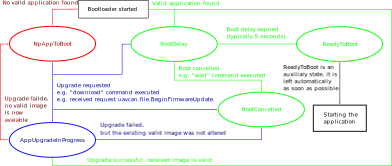
\includegraphics[width=1.1\textwidth]{bootloader_state_machine}}
	\caption{Bootloader state machine.\label{bootloader_state_machine}}
\end{figure}

\begin{ZubaxSimpleTable}{Bootloader states}{|c | l | X|}
State ID & State name & Comment \\
0 & NoAppToBoot & There is no valid application to boot; the bootloader will be waiting for commands forever.\\
1 & BootDelay & The bootloader will start the application in a few seconds, unless the boot is cancelled or a firmware update is requested.\\
2 & BootCancelled & There is a valid application to boot, however, boot was cancelled by an external command.\\
3 & AppUpgradeinProgress & Application is currently being upgraded. If interrupted, the bootloader will go into either \textbf{NoAppToBoot} or \textbf{BootCancelled}.\\
4 & ReadyToBoot & The application is about to boot. This state is very transient and is left automatically as soon as possible.
\end{ZubaxSimpleTable}

On Zubax~GNSS~2, the boot delay is set to 5 seconds.
The bootloader supports the following communication interfaces:

\begin{ZubaxSimpleTable}{Bootloader communication interfaces}{| l | l | X | X |}
Intreface & Parameters & Protocol & Note\\
USB & CDC ACM & YMODEM, XMODEM, XMODEM-1K (autodetect) & When connected, the DCD port is inactive\\
DCD port (UART) & 115200-8N1(fixed) & Same as USB CDC ACM & Available only while USB is disconnected\\
CAN1 bus & Autoconfigured & UAVCAN firmware update protocol & Always available on CAN1. CAN2 is not used in the bootloader.
\end{ZubaxSimpleTable}

As can be seen from the table, there are two families of protocols: serial and CAN based; both are reviewed below.

\section{Error codes}

The table below provides definitions for the well defined error codes that can be reported by the bootloader.

\begin{ZubaxSimpleTable}{Error codes}{| l | X |}
0 & Success.\\
1 & Unknown error.\\
9001 & Application ROM driver error: erase failed.\\
9002 & Application ROM driver error: write failed.\\
10001 & The current state of the bootloader does not permit the requested operation.\\
10002 & Application image is too large for the device. Download has been aborted.\\
10003 & Failed to write the next downloaded chunk of the application image into the ROM.\\
20001 & X/YMODEM interface write has timed out.\\
20002 & X/YMODEM retries exhausted.\\
20003 & X/YMODEM protocol error.\\
20004 & X/YMODEM transfer has been cancelled by the remote.\\
20005 & X/YMODEM remote has refused to provide the file.\\
30001 & UAVCAN service request has timed out.\\
30002 & UAVCAN file downloading has been interrupted.\\
32767 & Unknown error.
\end{ZubaxSimpleTable}

\section{LED indication}

While the bootloader is running, the LED indicators behave as follows:
\begin{itemize}
\item The status LED is always on, which is the main indicator that the bootloader, rather than the firmware, is currently running
\item The CAN1 LED behaves normally as a CAN bus activity and load indicator, blinking once for 25 milliseconds every time the CAN1 controller successfully transmits or receives a CAN frame.
\item The CAN2 LED displays one of the blinking patterns shown below, depending on which state the bootloader is in. While the bootloader is running, the state of this LED has no relation to the state of the redundant CAN interface (which is CAN2), since the bootloader makes no use of it.
\end{itemize}

\begin{ZubaxSimpleTable}{LED patterns during bootloader stage}{| l | X |}
Bootloader state & LED blinking pattern (step 50 ms) \\
NoAppToBoot  & 10 Hz (very quickly)\\
BootDelay, ReadyToBoot  & Turned off\\
BootCancelled &  1 Hz, short pulses (50 ms)\\
AppUpgradeInProgress & 1 Hz, long pulses (500 ms)
\end{ZubaxSimpleTable}

\section{Via USB/UART}

Once started, the bootloader exposes a CLI via either DCD port or USB. The USB is always preferred if it is connected to the host; otherwise the CLI falls back to the UART interface of the DCD port.

The CLI can be used to query the state of the bootloader, modify it, obtain the information about the running firmware, and upgrade it if necessary.

The CLI prompt is of the following format: \textbf{StateName>}, which features the human readable name of the current state of the bootloader, followed by the ASCII greater character (ASCII code 62), followed by a space. For example:  \textbf{BootDelay>}. Such prompt allows the user (or software) to easily identify the state of the bootloader.

\subsection{CLI commands}

\textbf{reboot}

Restarts the bootloader.

\textbf{zubax{\_}id}

This is the standard command supported by all products by Zubax Robotics that have a CLI. It takes no arguments, and outputs a YAML key-value dictionary containing the vital information about the device, the firmware it is running, unique ID, installed certificates of authenticity, version of the hardware, and possibly some other information. Aside from the standard fields, this command also provides at least the following fields in its output:

\begin{itemize}
\item \textbf{bl{\_}version} - bootloader version, major and minor.
\item \textbf{bl{\_}vcs{\_}commit} - build identifier of the bootloader.
\item \textbf{mode} - set to the string \textbf{bootloader} to indicate that the bootloader is running.
\end{itemize}

If there is a valid firmware, its version information will also be provided via the standard fields \textbf{fw{\_}version} and  \textbf{fw{\_}vcs{\_}commit}. If the bootloader could not find a valid firmware, these fields will be omitted.

\textbf{wait}

Do not boot the application. If the current state is \textbf{BootDelay}, the state will be switched to \textbf{BootCancelled}. In all other states the command will have no effect.

\textbf{download}

Start the serial receiver and prepare to receive the new firmware image as a flat binary via the serial link using either YMODEM, XMODEM, or XMODEM-1K. The bootloader will automatically detect which protocol to use. According to the YMODEM specification, if no transfer was initiated by the host within one minute, the command will exit with an error. Possible error codes are defined in the table above.

Note that while this command is running, the CLI will be unavailable, since the same serial link will be temporarily occupied by the file transfer protocol.

If the YMODEM protocol is used, the file name field in the transfer header packet will be ignored.

There are heaps of software products and scripts that support these file transfer protocols. For instance, the popular program \textbf{sz} (available on most Linux distributions) can be used as follows:
\begin{minted}[linenos = false]{bash}
sz -vv --ymodem --1k \$file > \$port < \$port
\end{minted}

\section{Via CAN bus}

The bootloader supports the UAVCAN firmware update protocol. Please refer to the UAVCAN specification for theory.

The bootloader only utilizes the primary CAN interface, which is CAN1. The redundant interface CAN2 remains in the passive mode while the bootloader is running. It is therefore required that if there is only one interface in use, it must be CAN1.

The following table describes the mapping from the bootloader states to the UAVCAN node status codes:

\begin{ZubaxSimpleTable}{Bootloader states and UAVCAN node status codes}{| X | X | X |}
Bootloader state & UAVCAN node mode & UAVCAN node health\\
NoAppToBoot & SOFTWARE{\_}UPDATE & ERROR\\
BootDelay, ReadyToBoot & MAINTENANCE & OK\\
BootCancelled & MAINTENANCE & WARNING\\
AppUpgradeInProgress & SOFTWARE{\_}UPDATE & OK
\end{ZubaxSimpleTable}

The vendor specific status code of the node status message contains the status code of the last attempt to upgrade the firmware. Please refer to the error code table provided above.

\subsection{Supported messages}
\begin{ZubaxSimpleTable}{Supported messages}{| l | l | l | l |}
Data type & Direction & Period & Transfer priority \\
\texttt{uavcan.protocol.NodeStatus} & Output & 1 Hz & 24(low) \\
\texttt{uavcan.protocol.debug.LogMessage} & Output & Aperiodic & 31(lowest) \\
\texttt{uavcan.protocol.dynamic{\_}node{\_}id.Allocation} & Input/Output & Aperiodic & 24 (low)
\end{ZubaxSimpleTable}

\begin{ZubaxSimpleTable}{Supported messages annotation}{| l | X |}
Data type & Note\\
\texttt{uavcan.protocol.NodeStatus} & Refer to the bootloader state mapping table.\\
\texttt{uavcan.protocol.debug.LogMessage} & Used to report the application upgrade progress and status in a human readable form.\\
\texttt{uavcan.protocol.dynamic{\_}node{\_}id.Allocation} & Used only during initialization, if the application did not provide a specific node ID to use.
\end{ZubaxSimpleTable}

\subsection{Supported services}

\begin{ZubaxSimpleTable}{Supported servers}{| l | X |}
Data type & Note\\
uavcan.protocol.GetNodeInfo & The nested structure  \textbf{uavcan.protocol.SoftwareVersion} is populated only if there is a valid application.\\
uavcan.protocol.RestartNode & Restarts the bootloader.\\
uavcan.protocol.file.BeginFirmwareUpdate & Initiates the firmware update process, unless it was initiated earlier before the application has rebooted into the bootloader.
\end{ZubaxSimpleTable}

\begin{ZubaxSimpleTable}{Supported clients}{| l | l | l | X |}
Data type & Response timeout & Transfer priority & Note \\
uavcan.protocol.file.Read & 1 second & 24(low) & Used to download the application image file from the specified file server.
\end{ZubaxSimpleTable}

The interval at which the file read requests are issued while downloading the application image is defined by the following formula (all units SI):

\begin{equation}
\text{last{\_}response{\_}latency} + 1 / (1 + \text{can{\_}bus{\_}bit{\_}rate} / 65536)
\end{equation}

This formula, combined with the low transfer priority, allows the bootloader to avoid congestion of the CAN bus while downloading the firmware image.

\chapter{Mechanical characteristics}\label{sec:mechanical}

The drawing below documents the basic mechanical characteristics of Zubax~GNSS~2,
such as the placement of connectors and mounting holes.

\begin{figure}[!hbt]
    \center
	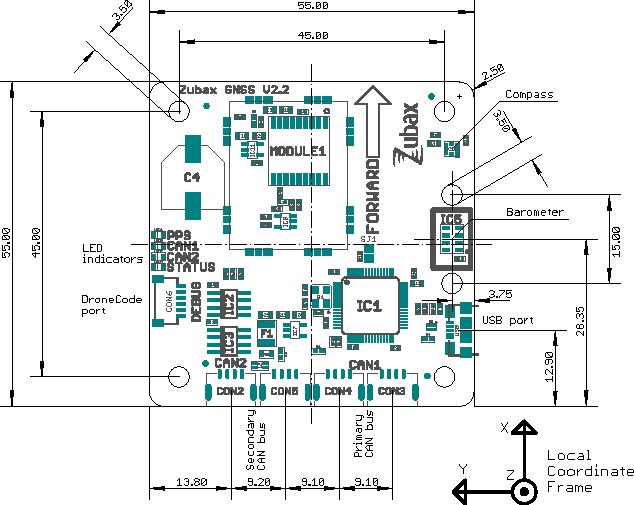
\includegraphics[width=1\textwidth]{GNSS2_drawing}
	\caption{GNSS2 drawing.\label{drawing}}
\end{figure}


\end{document}
